\documentclass[a4paper,11pt]{article}
\usepackage[utf8]{inputenc}
\usepackage{graphicx}
\usepackage[UKenglish]{datetime}
\usepackage[top=1in, bottom=1in, right=1in, left=1in]{geometry}
\usepackage{pdfpages}
\usepackage{hyperref}

\begin{document}

\author{Minh Le Kieu \and Koen H. van Dam\and Jason Thompson \and Nick Malleson \and Alison Heppenstall \and Jiaqi Ge}
\title{International Workshop on \\ Agent-Based Modelling of Urban Systems (ABMUS) \\ Proceedings: 2022}
\date{Tuesday 10th May 2022}

\maketitle

ABMUS is a workshop where urban and geo-spatial modellers get together in a focused session, during the International Conference on Autonomous Agents and Multiagent Systems (AAMAS). The central goal of this workshop is to bring together the community of researchers and practitioners who use agent-based models and multi-agent systems to understand and manage cities and urban infrastructure systems. Through the exchange of ideas and state-of-the-art within this area, we will pool together current thinking to discuss avenues of fruitful research and methodological challenges we face in building robust, realistic, and trusted models of urban systems. Drawing from recognised challenges faced by the modeling community through the COVID-19 pandemic and similar public policy crises, the overarching theme for the workshop this year will be ‘\textbf{Trust, Transparency and Translation}’. Participants will be asked to describe how their models are creating a bridge between the synthetic and real worlds, and making their way into real-world policy and decision-making. This year, we invite presentations that describe how researchers construct their models, demonstrate results, work with policy and decision-makers, and how these processes either facilitate or hinder the process of urban systems model building from the modeller's perspective. We will discuss challenges associated with model development, data interoperability, consistent representation of space and time, as well as developments in interfaces and stakeholder engagement.

Further details are available at: \url{http://modelling-urban-systems.com/abmus2022/}

\newpage
\tableofcontents

\newpage

\section{Session 1: Methodology}

\subsection{Synthetic generation of individual transport data: the case of Smart Card data
 \\ Minh Kieu, Iris Meredith and Andrea Raith}
 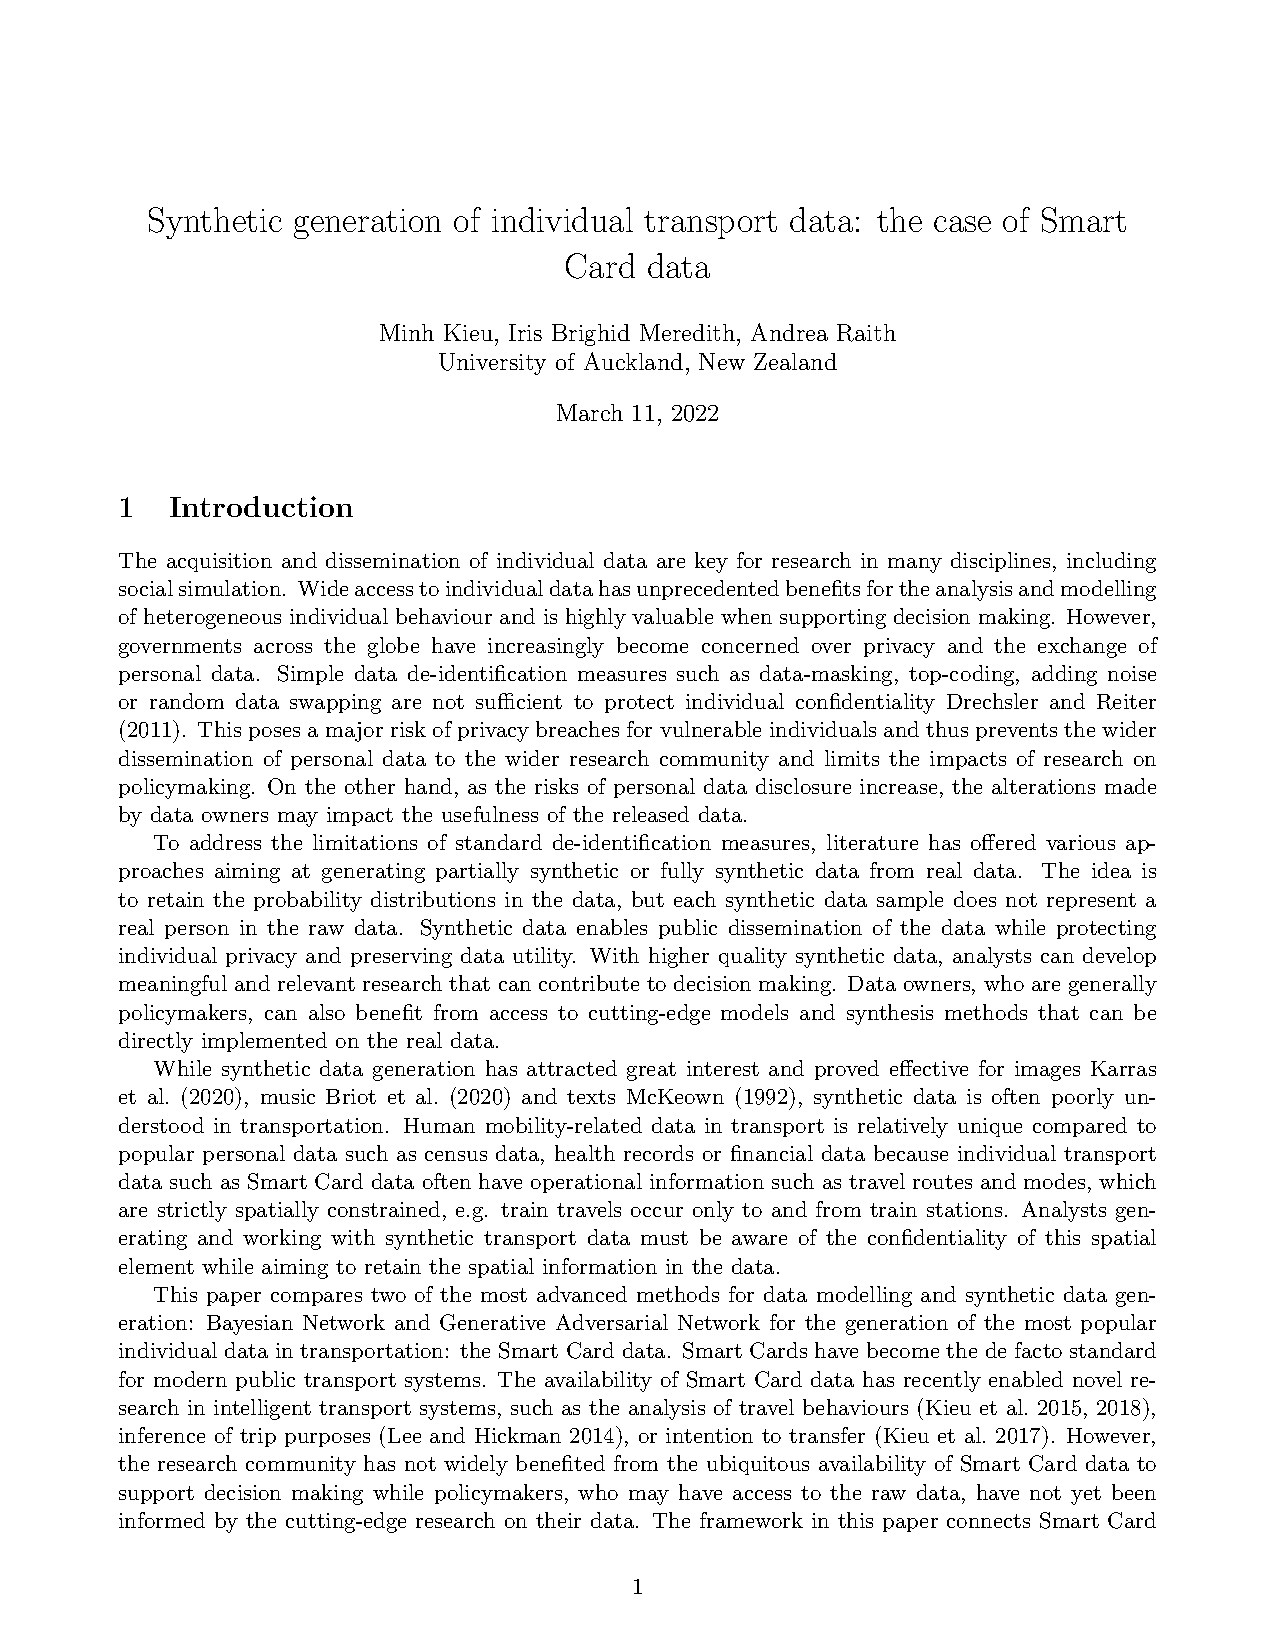
\includepdf[pages=-]{ABMUS2022_paper_8.pdf}

\subsection{Data-driven agent-based model development to support human-centric TOD design \\ Liu Yang and Koen van Dam. }
 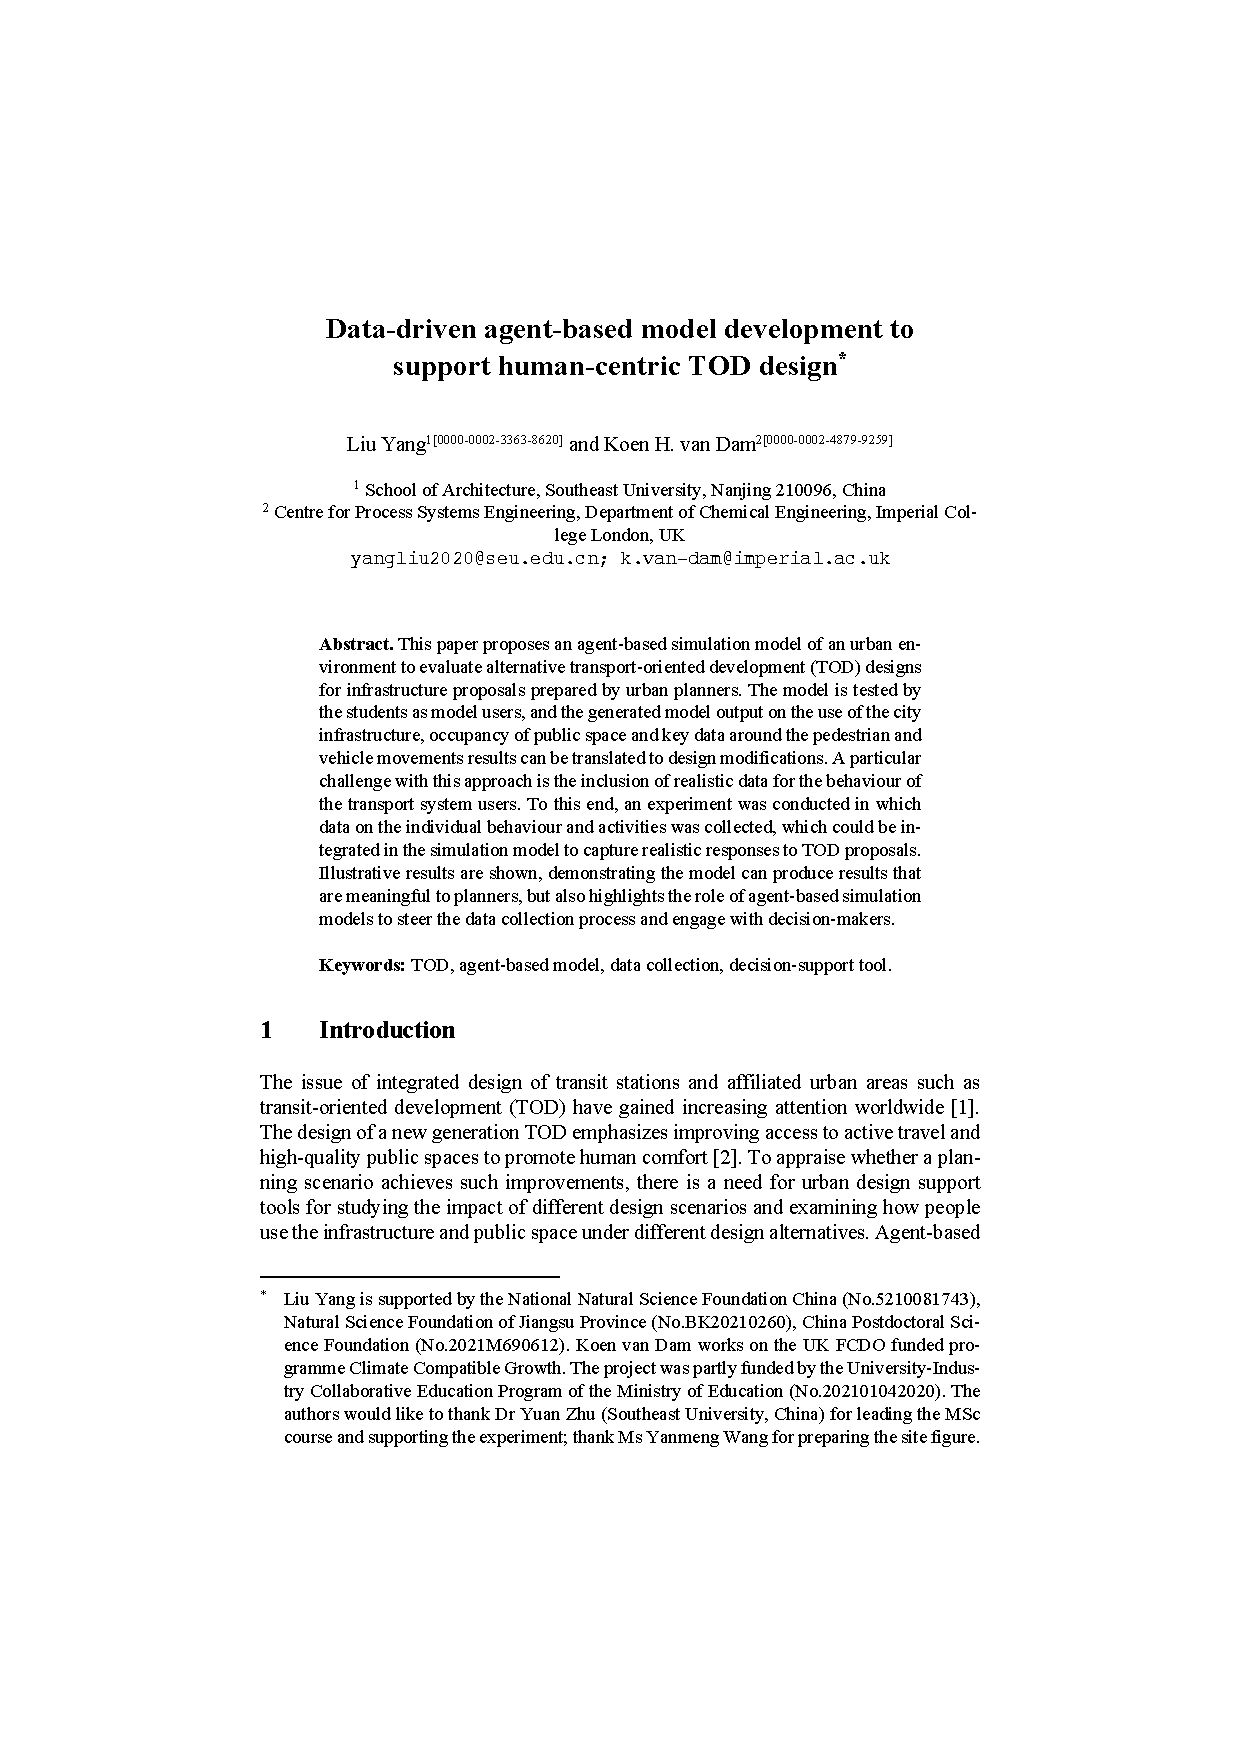
\includepdf[pages=-]{ABMUS2022_paper_5.pdf}

\subsection{AgentsX.jl — An Extended Julia Framework for Exploring Urban and Social Systems \\ Rajith Vidanaarachchi, Jason Thompson, Branislava Godic and Rod McClure}
 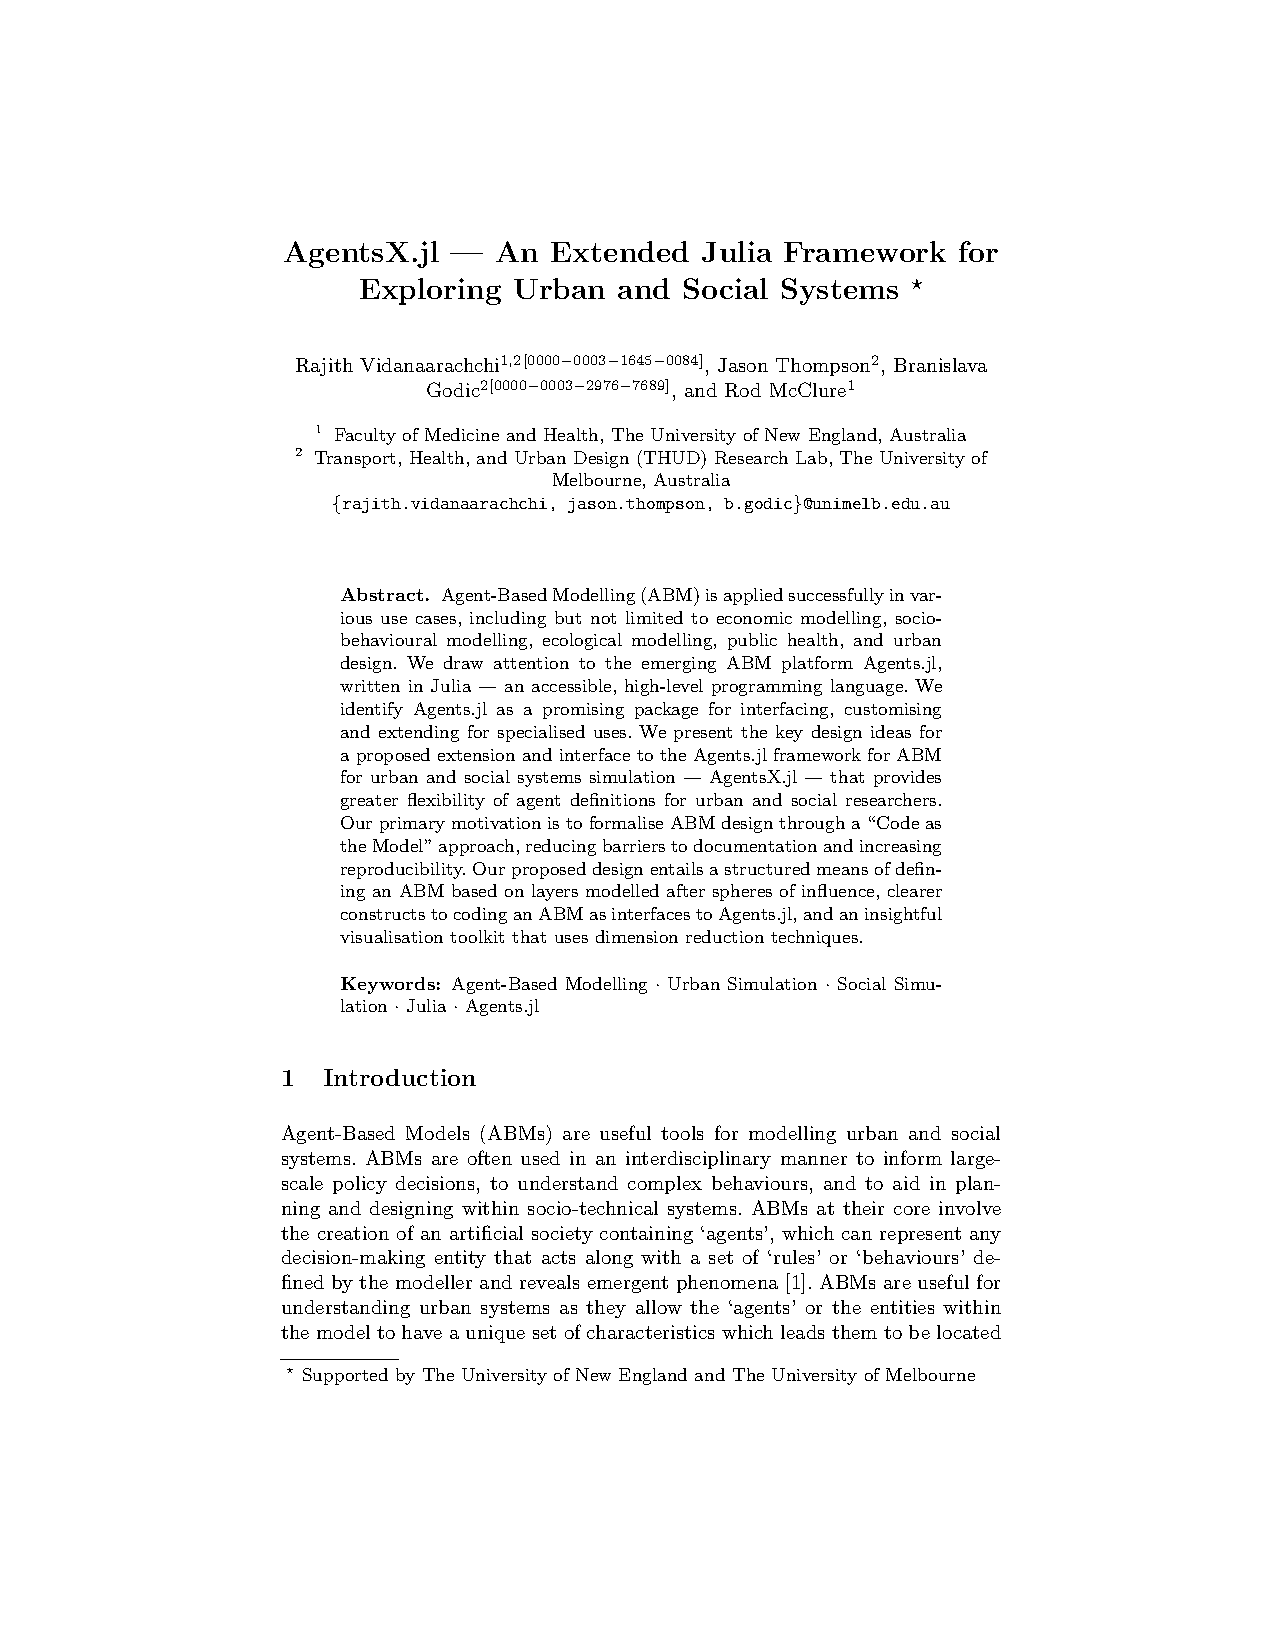
\includepdf[pages=-]{ABMUS2022_paper_9.pdf}

\subsection{Simulating civil emergency evacuation with Inverse Generative Social Science \\ Gayani Senanayake and Minh Kieu}
 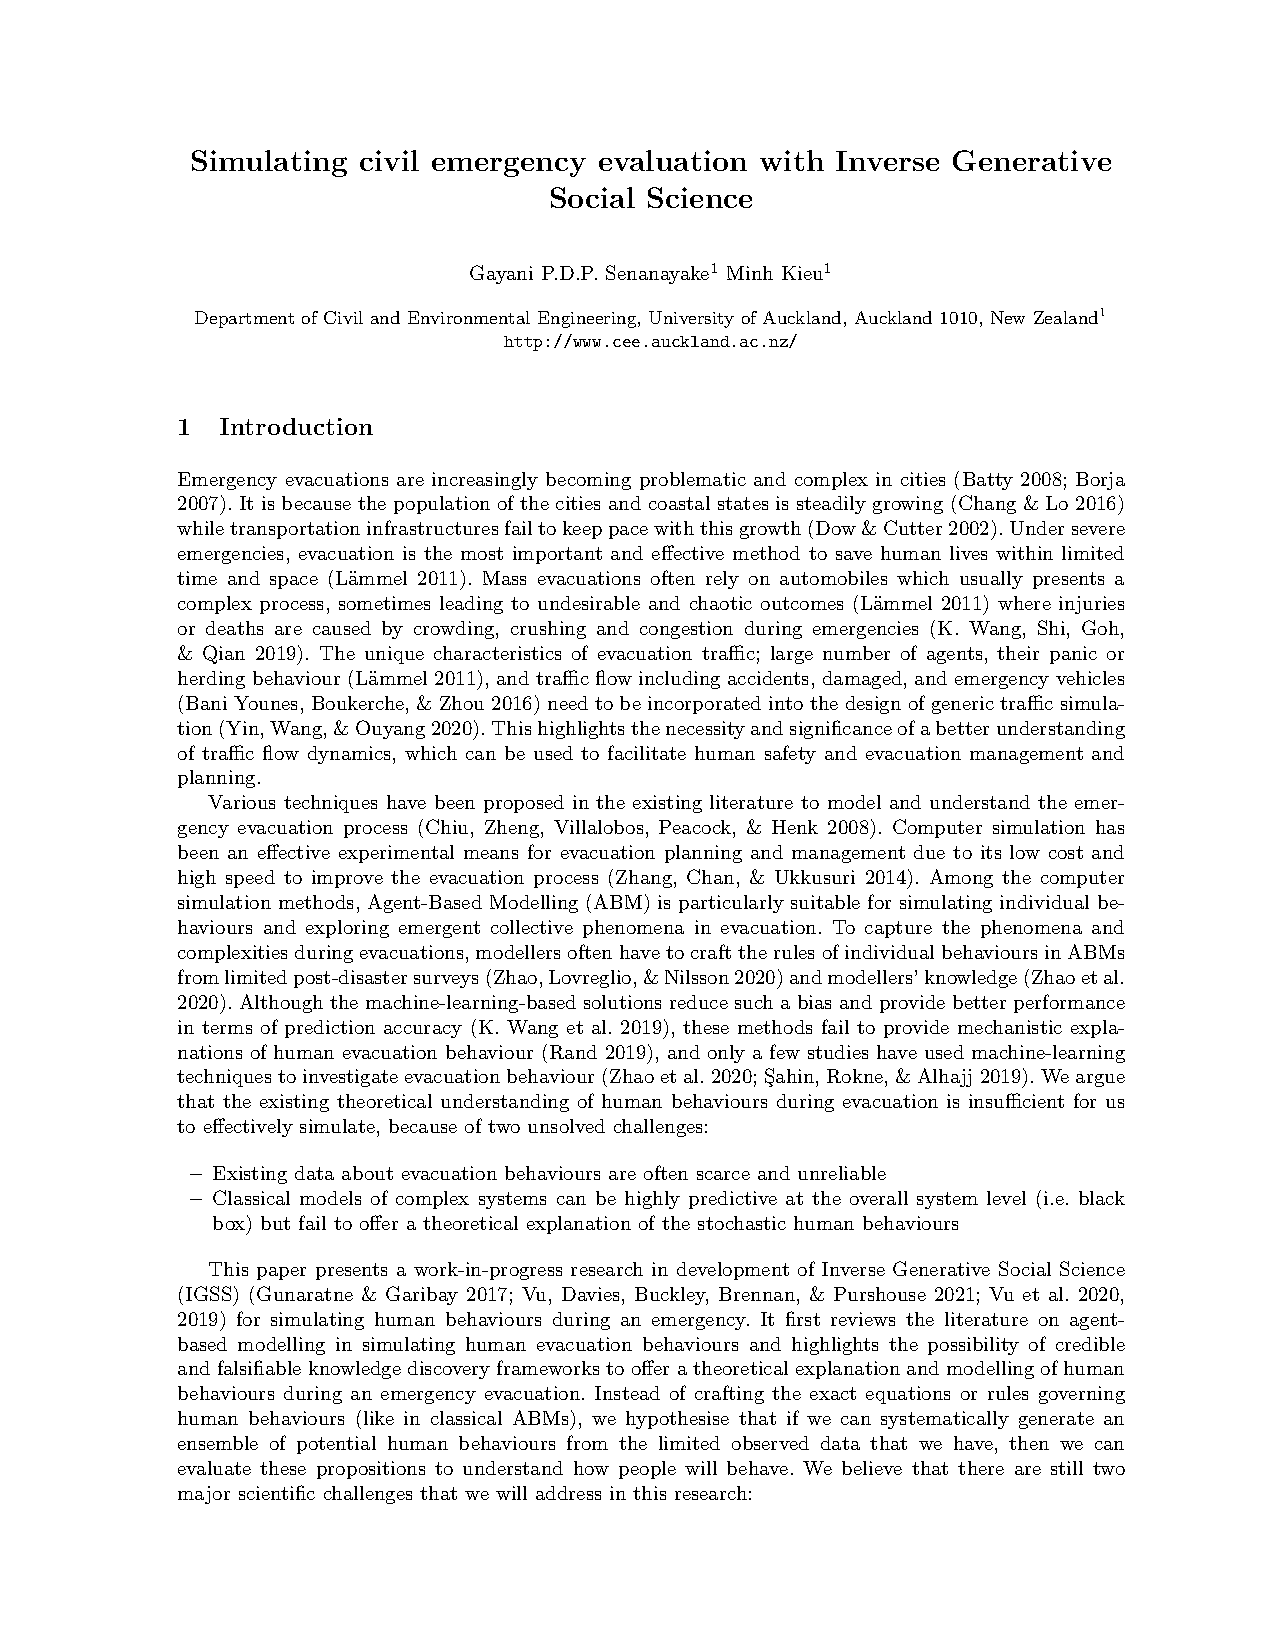
\includepdf[pages=-]{ABMUS2022_paper_12.pdf}


\section{Session 2: Urban Development}

\subsection{No Hope for First-Time Buyers? Towards Agent-Based Market Analysis of Urban Housing Balance \\ Erik Wiegel and Neil Yorke-Smith. }
 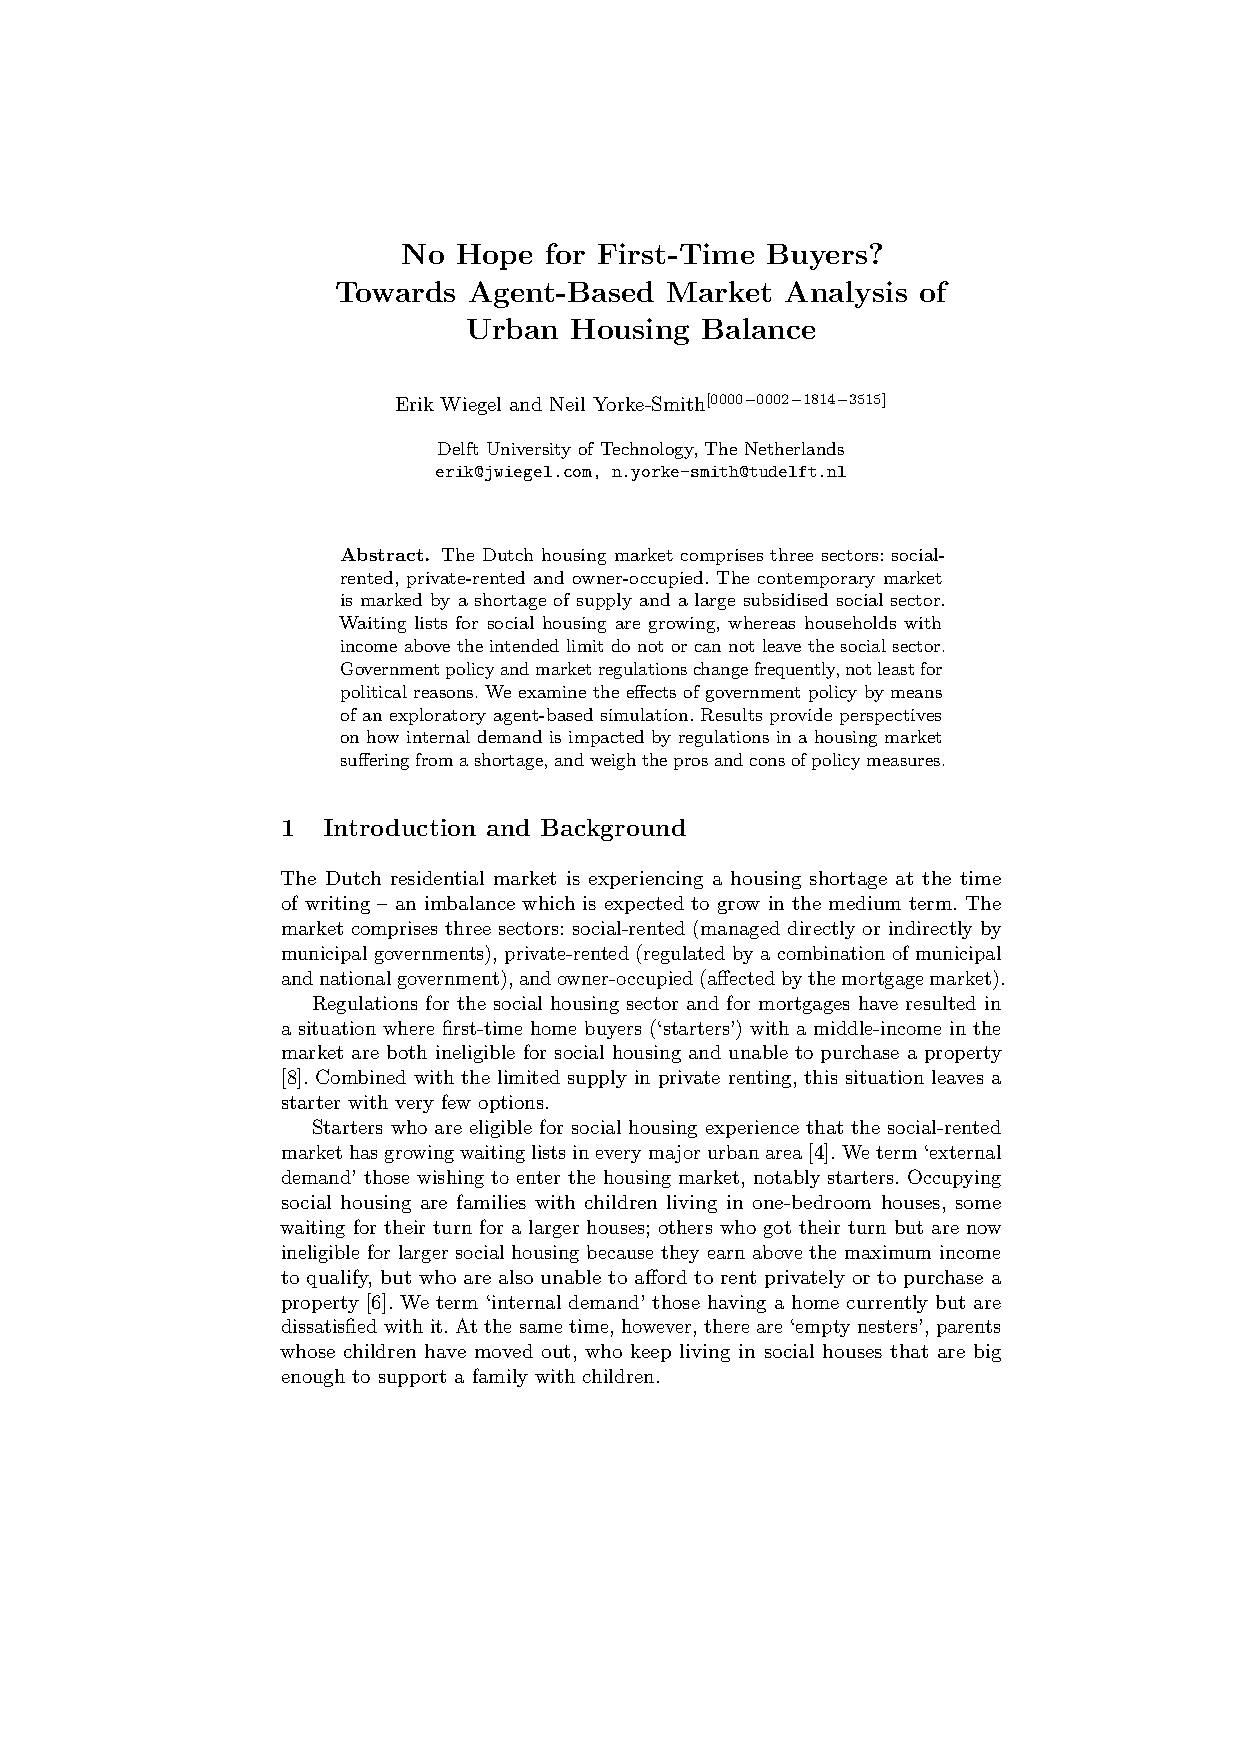
\includepdf[pages=-]{ABMUS2022_paper_1.pdf}
 
 \subsection{Agent-Based Modelling of People's Behaviour in Public Parks \\ Sabine Timpf and Marie-Rose Degg. }
 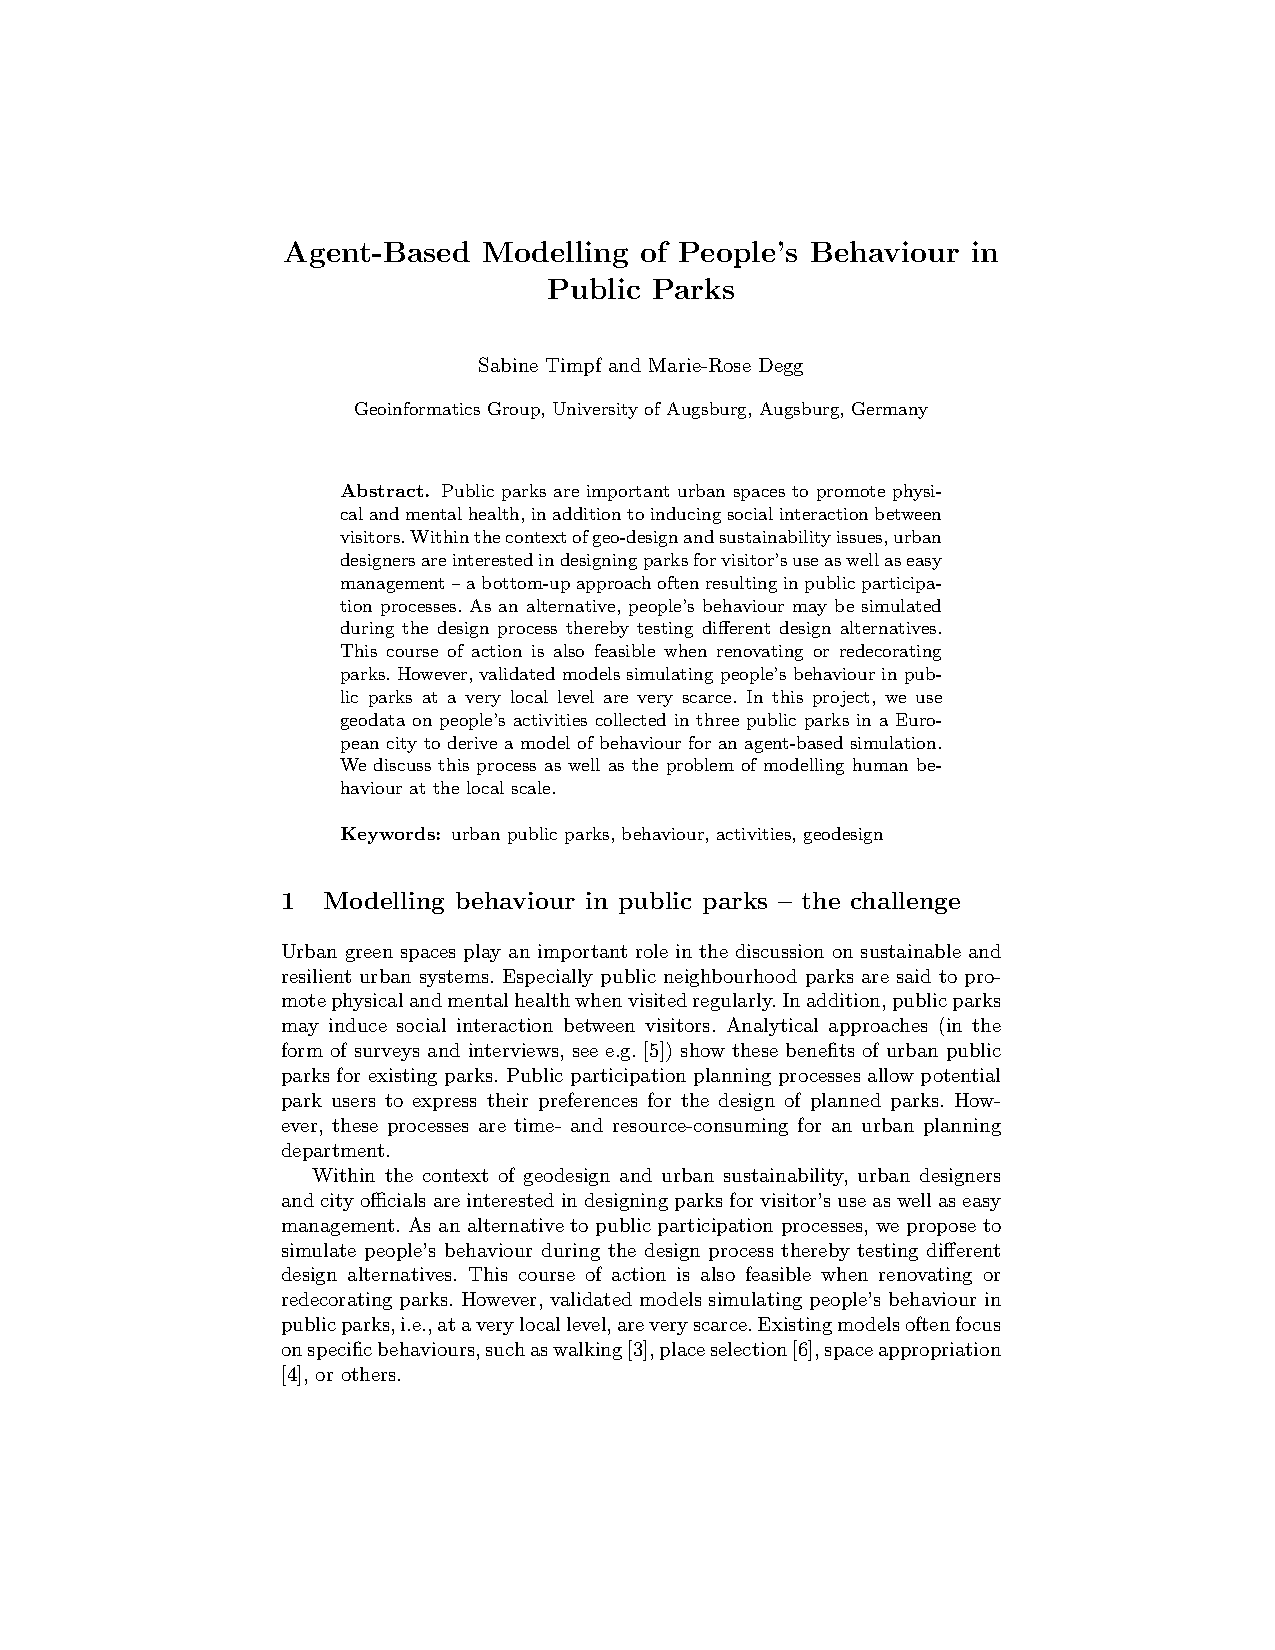
\includepdf[pages=-]{ABMUS2022_paper_11.pdf}
 
 \subsection{An agent-based model of greening a city for reducing pluvial flooding at a cultural heritage site \\ Emily West, Rembrandt Koppelaar, Aitziber Egusquiza Ortega, Angela Santangelo and Eleonora Melandri.}
 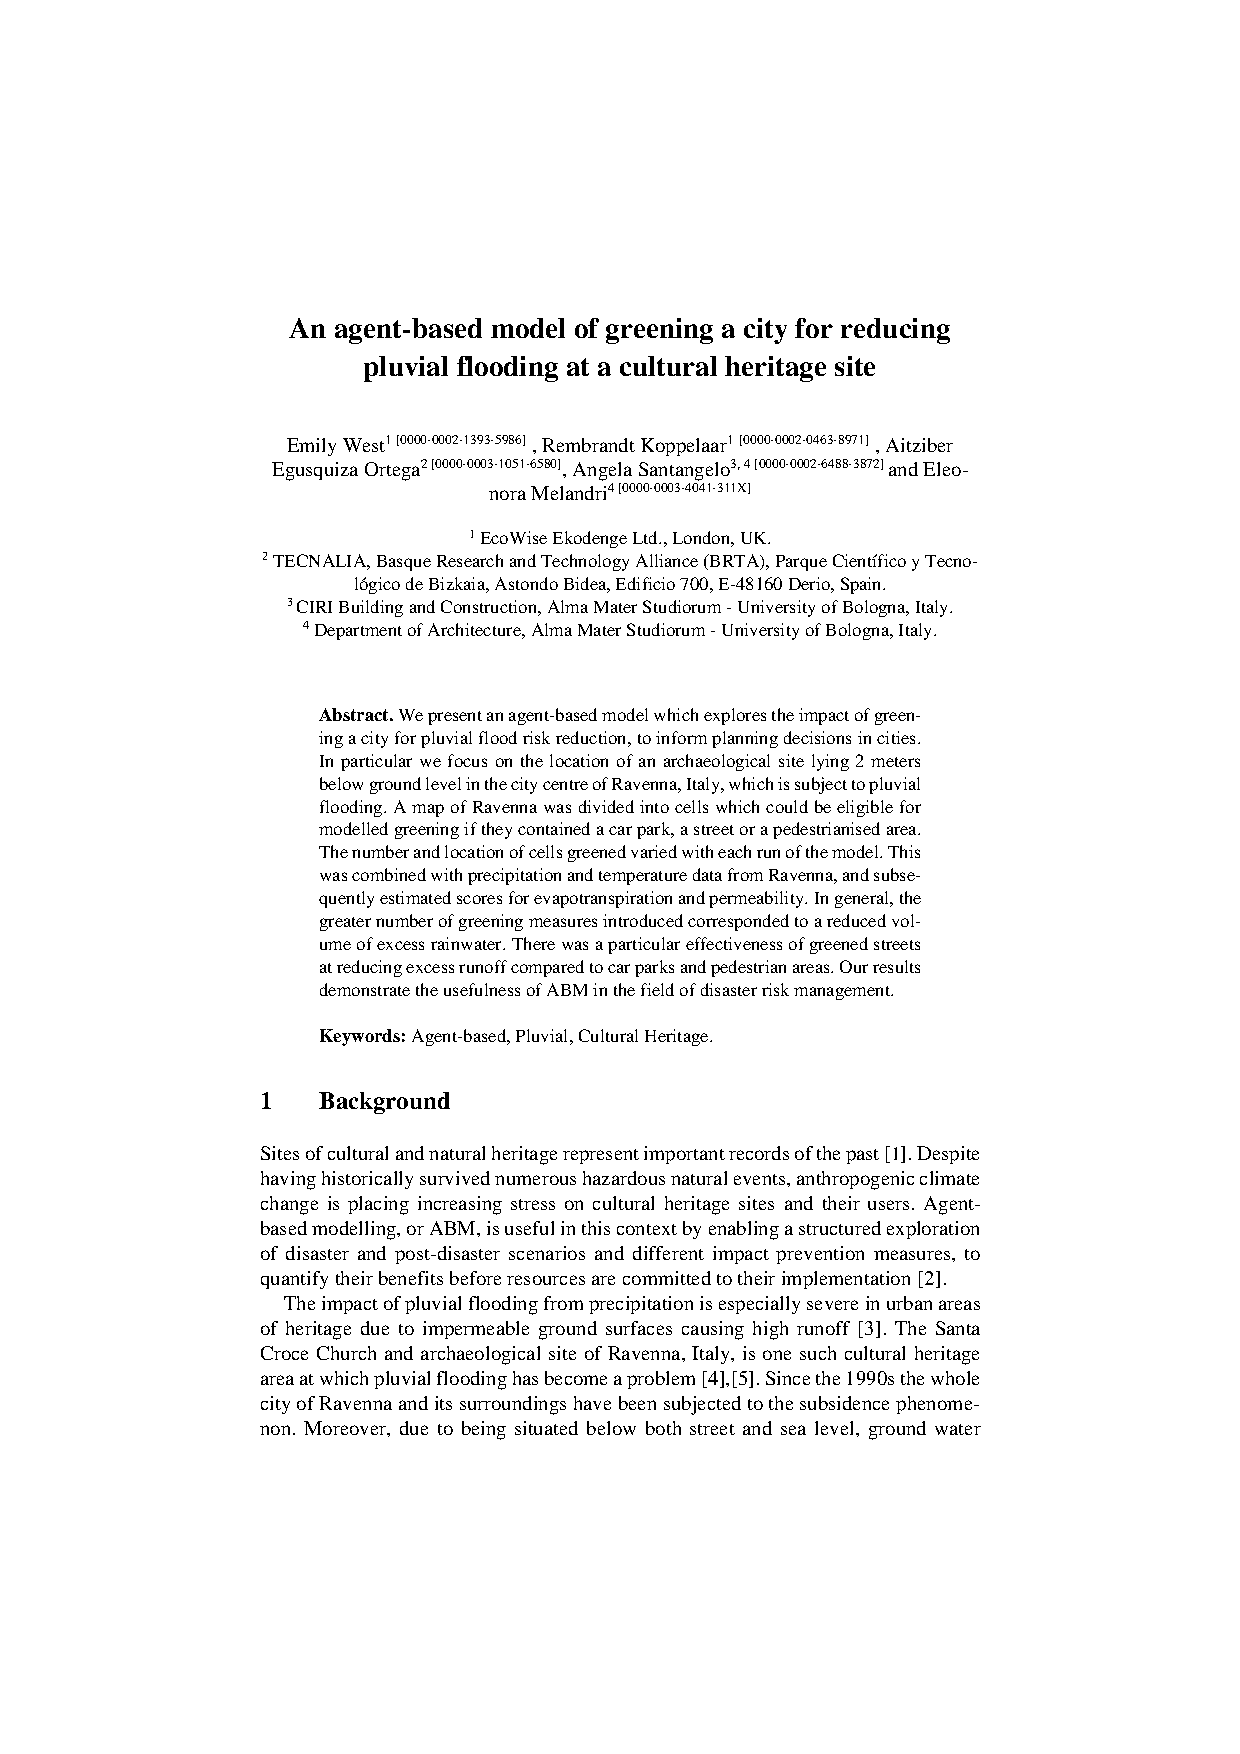
\includepdf[pages=-]{ABMUS2022_paper_2.pdf}
 
 \subsection{Real World Traffic Optimization by Reinforcement Learning: A Concept \\ Henri Meeß, Jeremias Gerner, Daniel Hein, Stefanie Schmidtner and Gordon Elger. }
 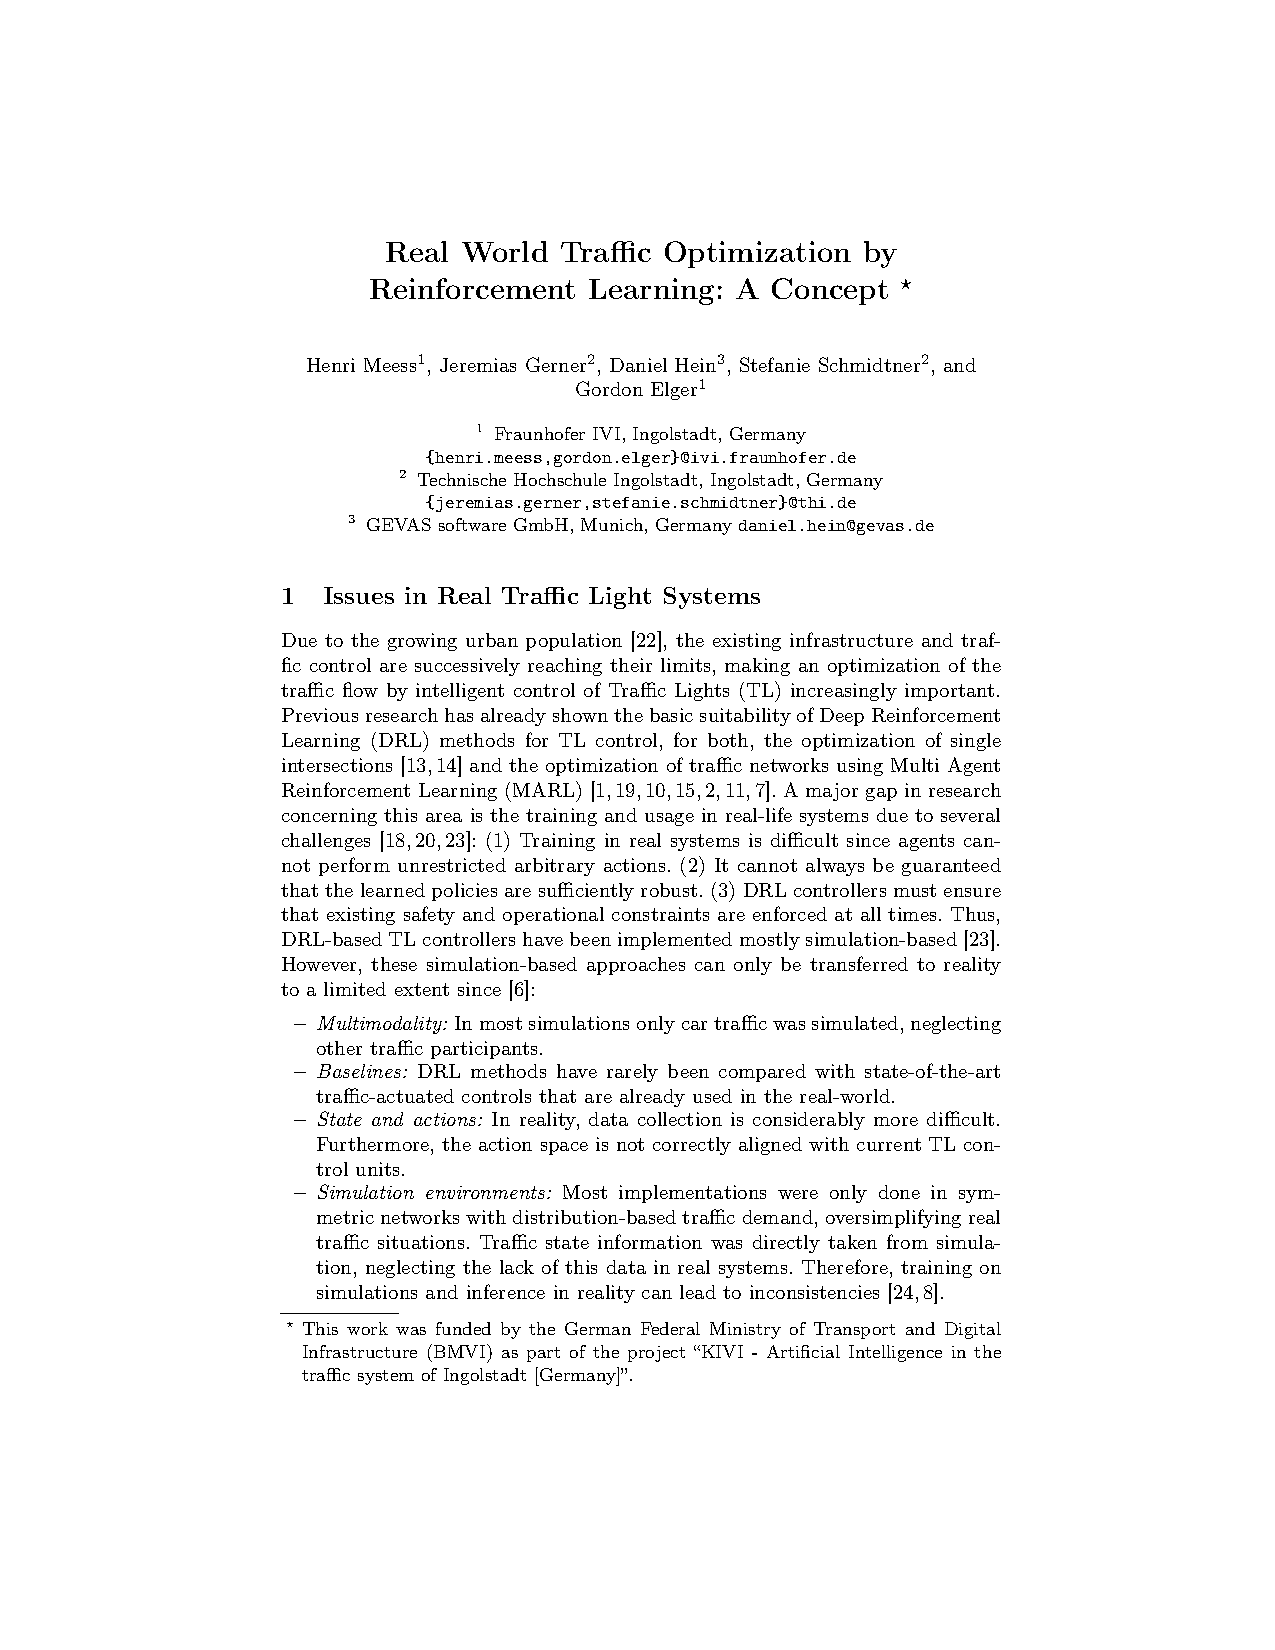
\includepdf[pages=-]{ABMUS2022_paper_4.pdf}

\section{Session 3: Transport}

\subsection{Transport electrification and fast-charging expansion: A case study in Alaska \\ Ilya Turchaninov, Koen van Dam, Gonzalo Bustos Turu and Salvador Acha.}
 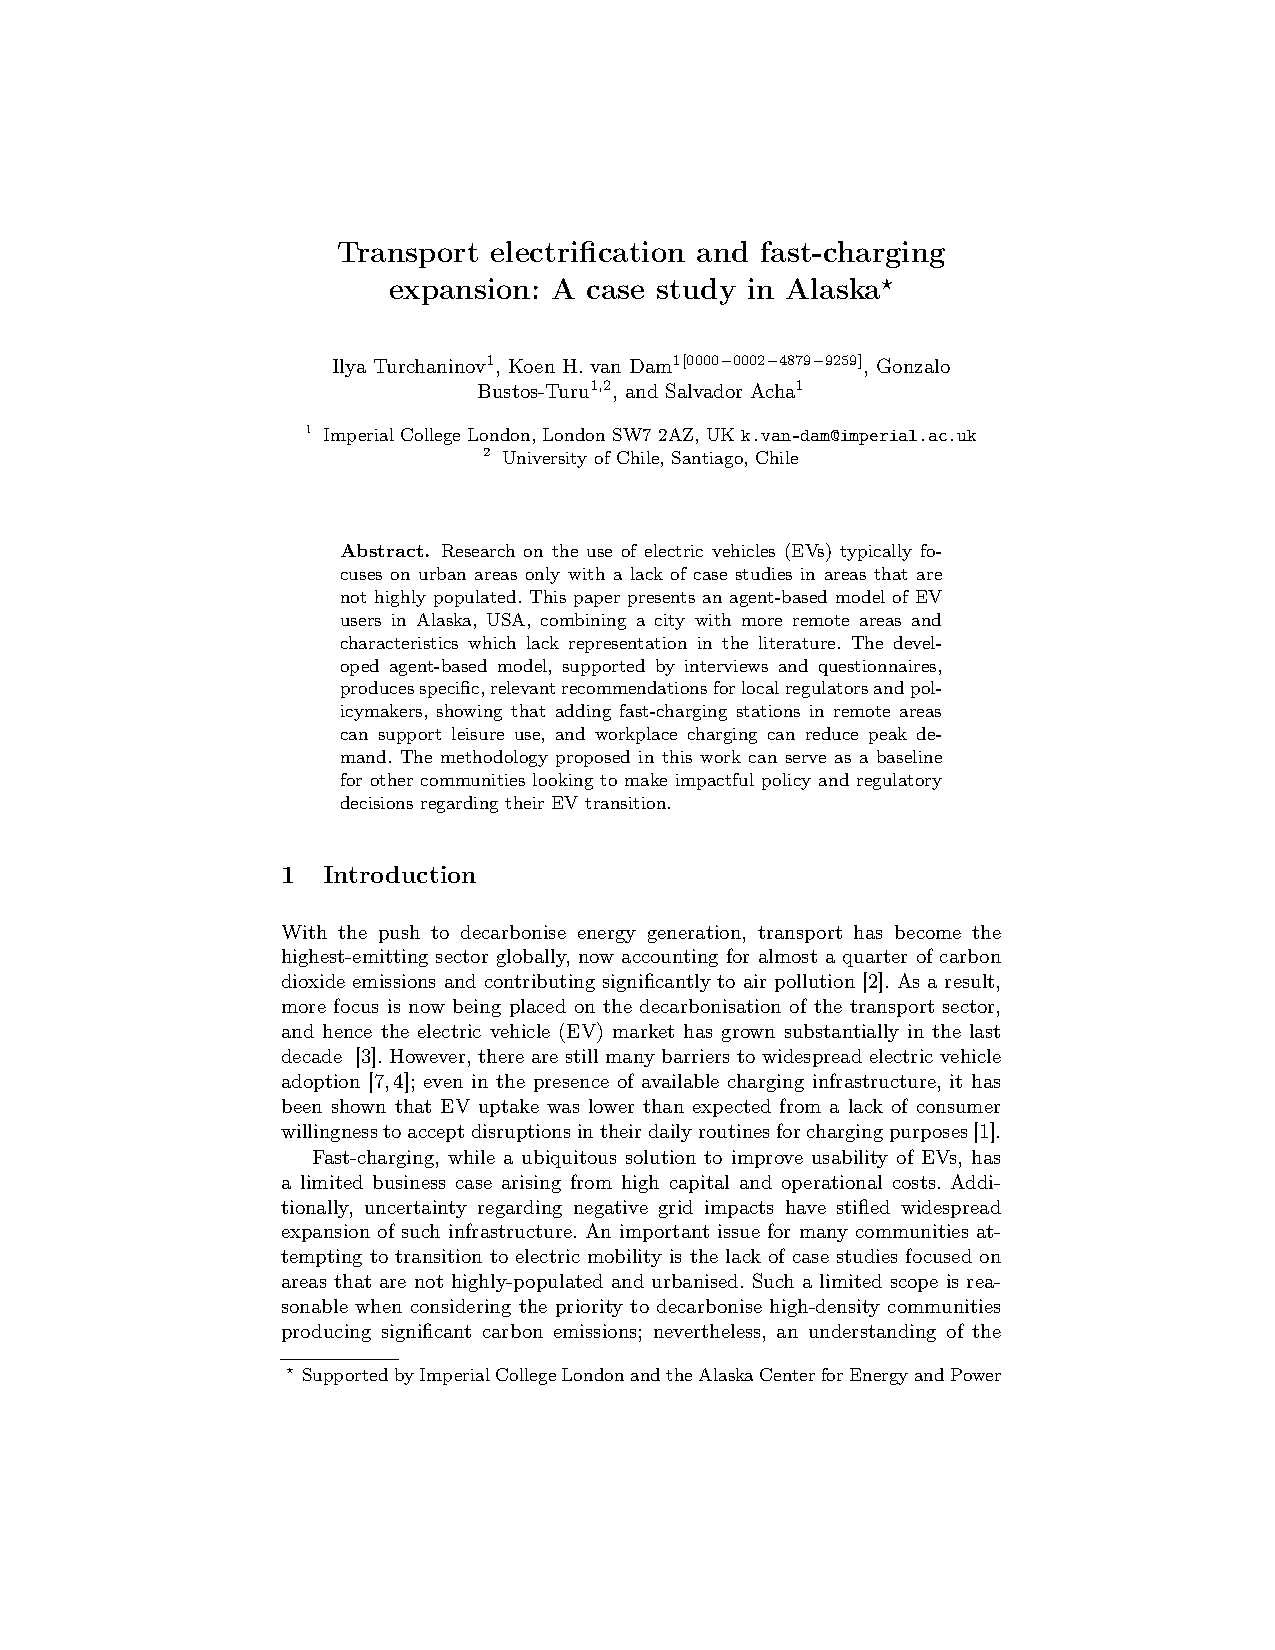
\includepdf[pages=-]{ABMUS2022_paper_10.pdf}
 
 \subsection{Learning a Robust Multiagent Driving Policy for Traffic Congestion Reduction \\ Yulin Zhang, William Macke, Jiaxun Cui, Daniel Urieli and Peter Stone}
 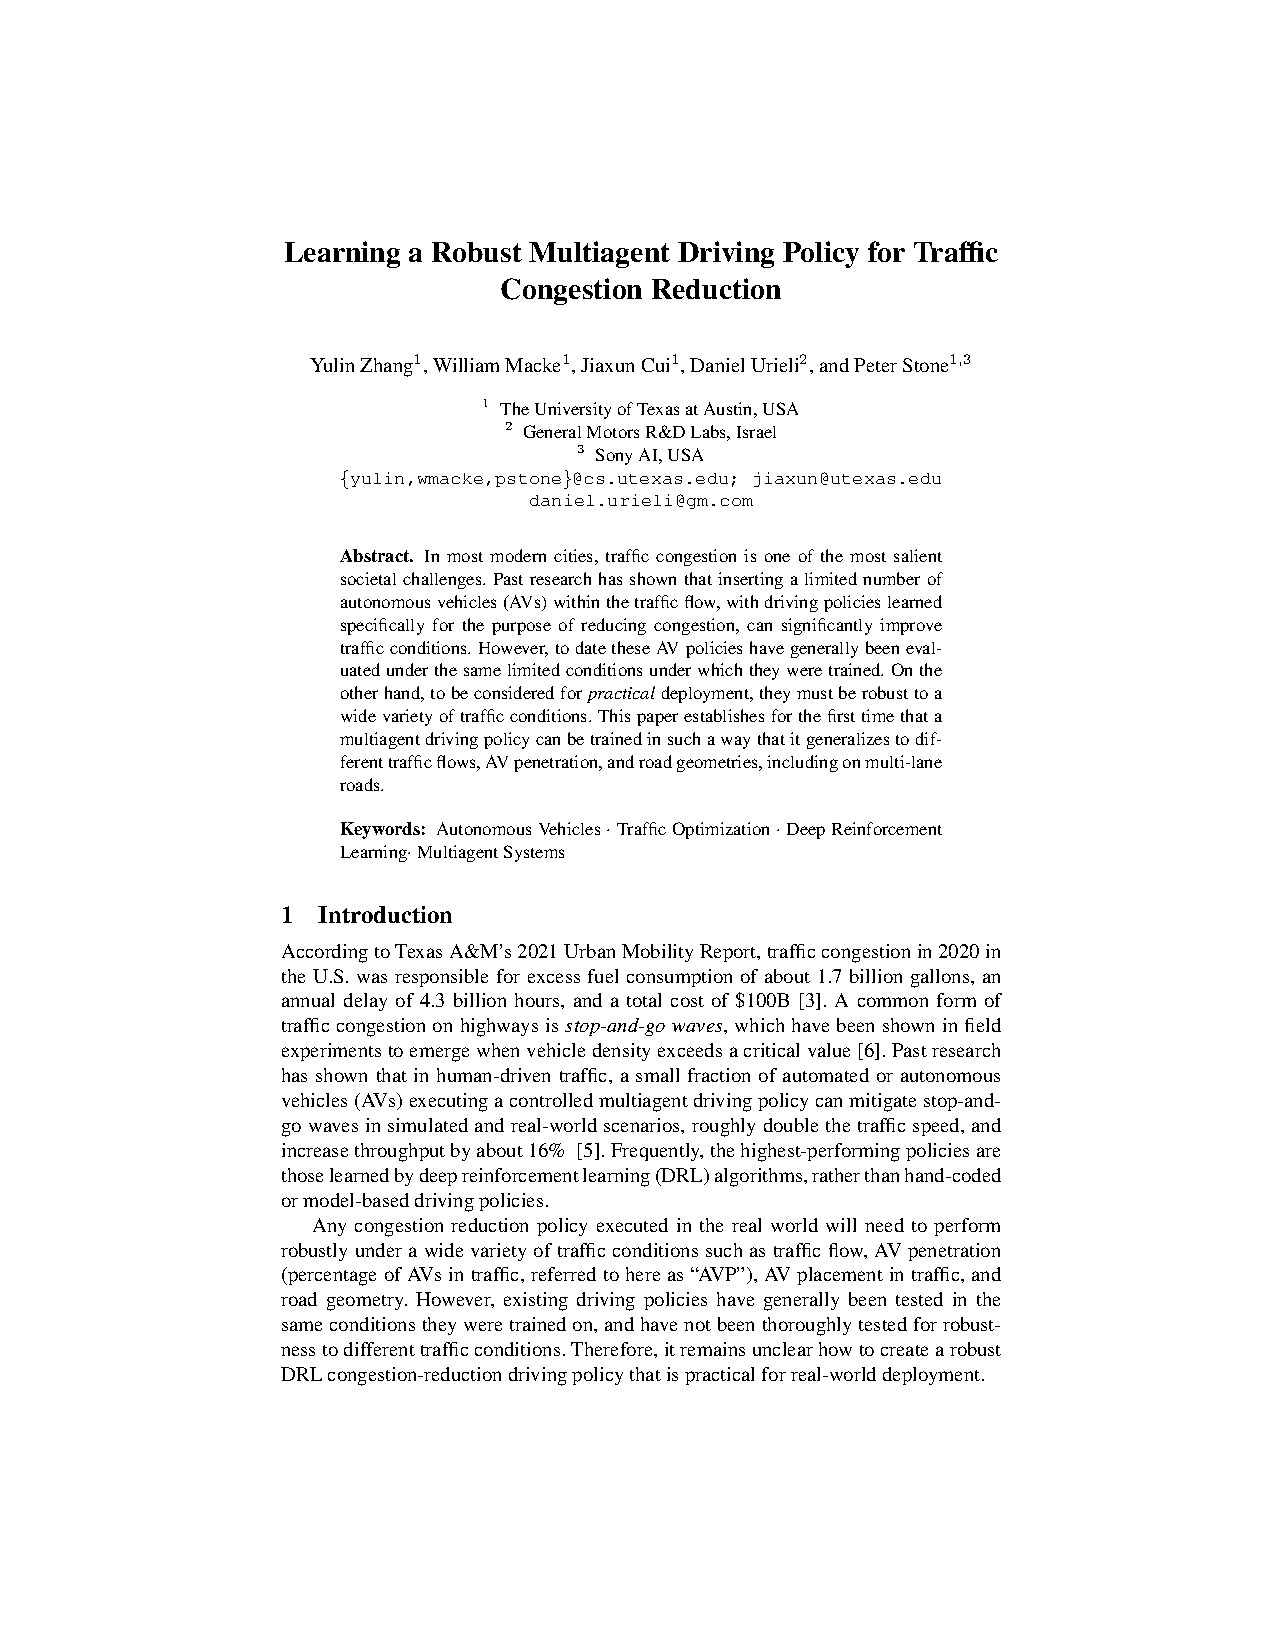
\includepdf[pages=-]{ABMUS2022_paper_3.pdf}
 
 \subsection{Preference-Aware Dynamic Ridesharing \\ Yi Cheng Ong, Nicos Protopapas, Vahid Yazdanpanah, Enrico H. Gerding and Sebastian Stein}
 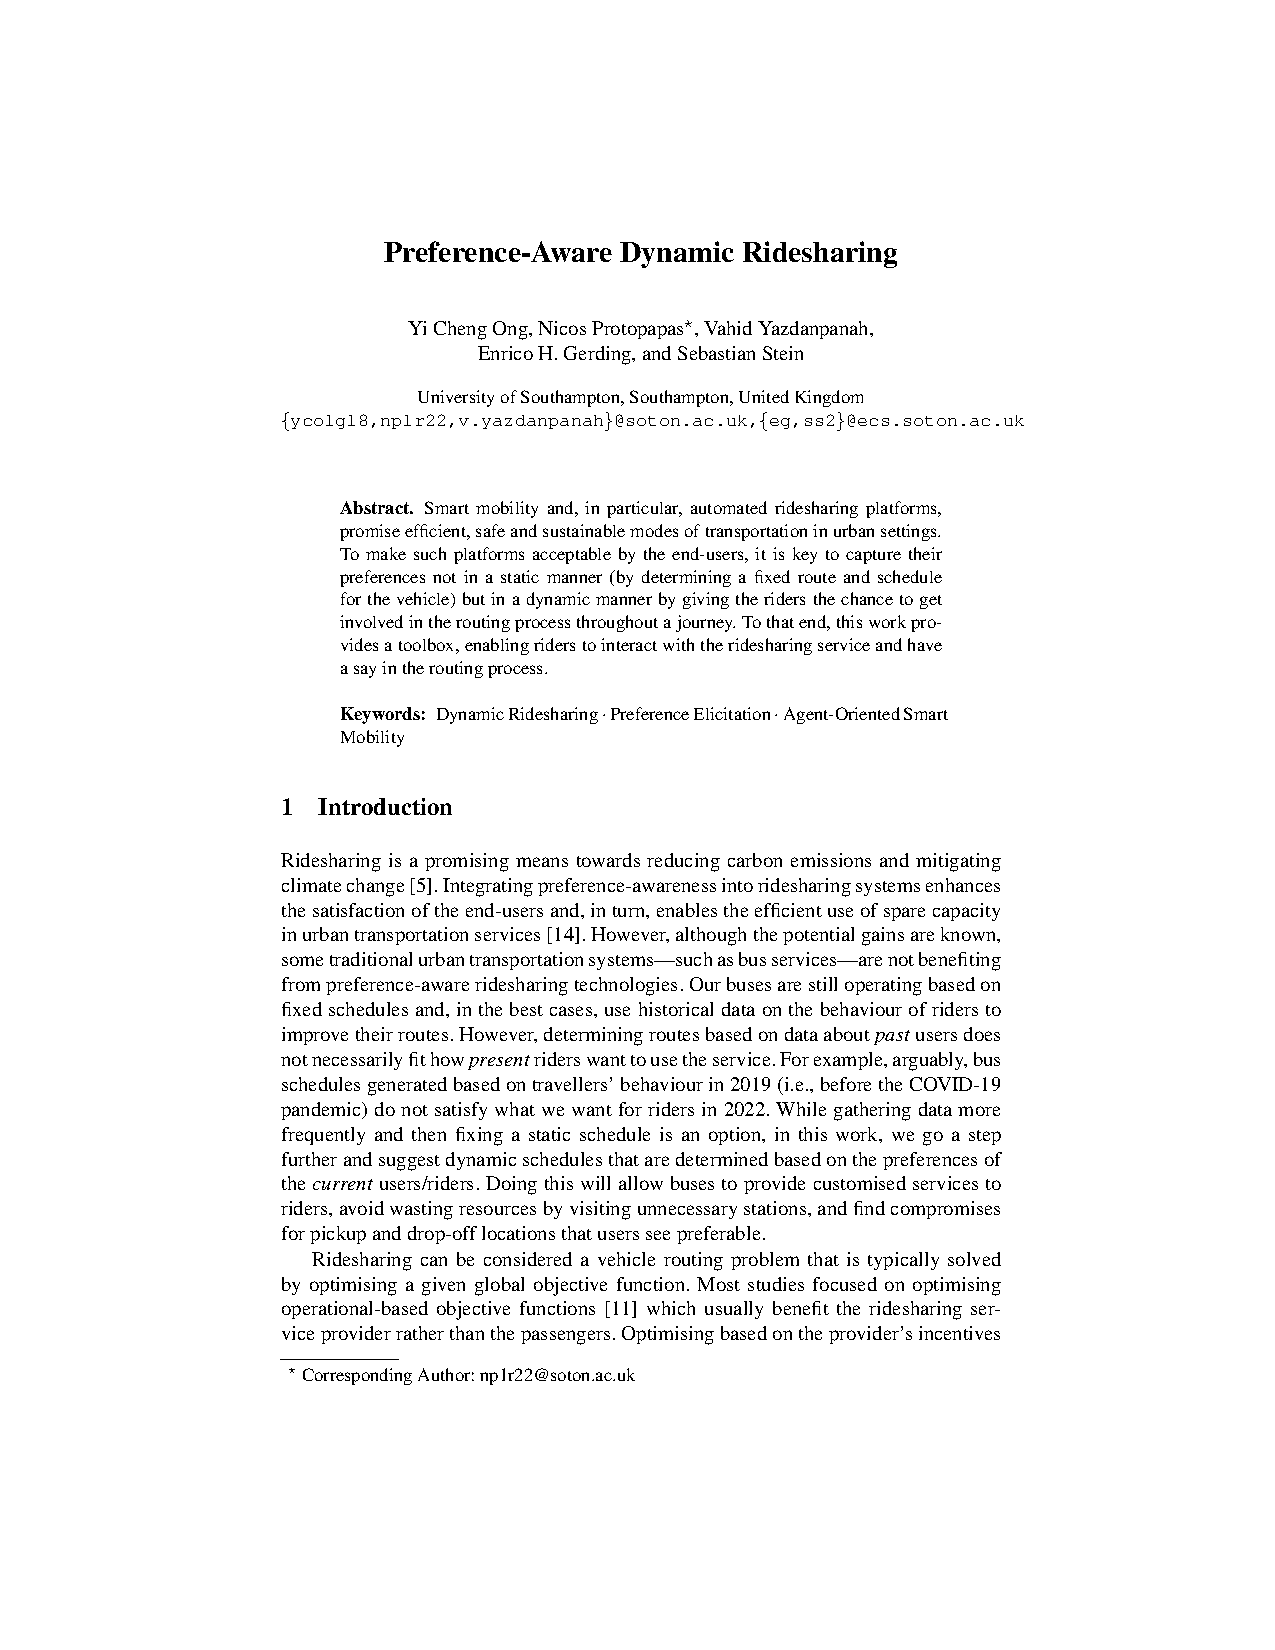
\includepdf[pages=-]{ABMUS2022_paper_6.pdf}
 
 \subsection{Multi-Agent Traffic Signal Control via Distributed RL with Spatial and Temporal Feature Extraction \\ Yifeng Zhang, Mehul Damani and Guillaume Sartoretti}
 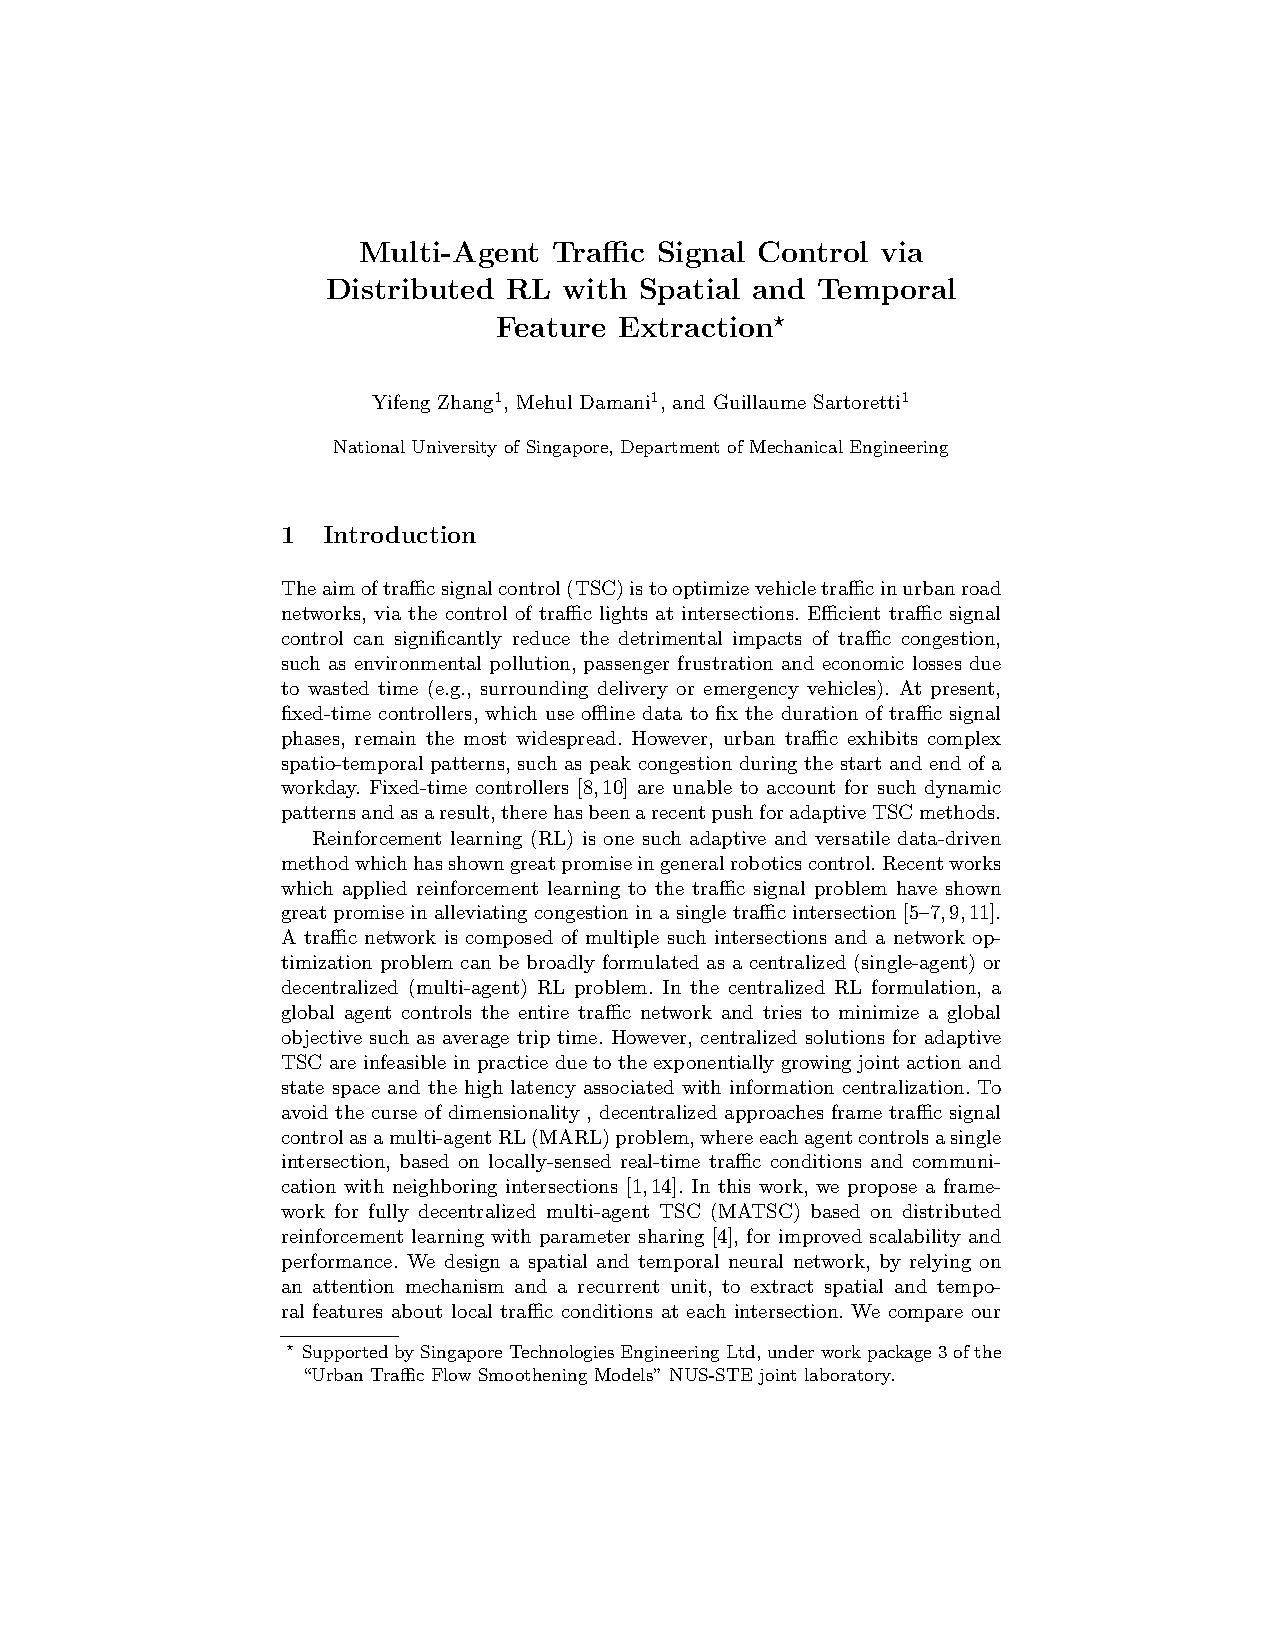
\includepdf[pages=-]{ABMUS2022_paper_7.pdf}
 

\end{document}
